\documentclass{standalone}
\usepackage{tikz}
\usetikzlibrary{patterns, positioning}
\usepackage[sfdefault]{ClearSans} %% option 'sfdefault' activates Clear Sans as the default text font
\usepackage[T1]{fontenc}

\begin{document}
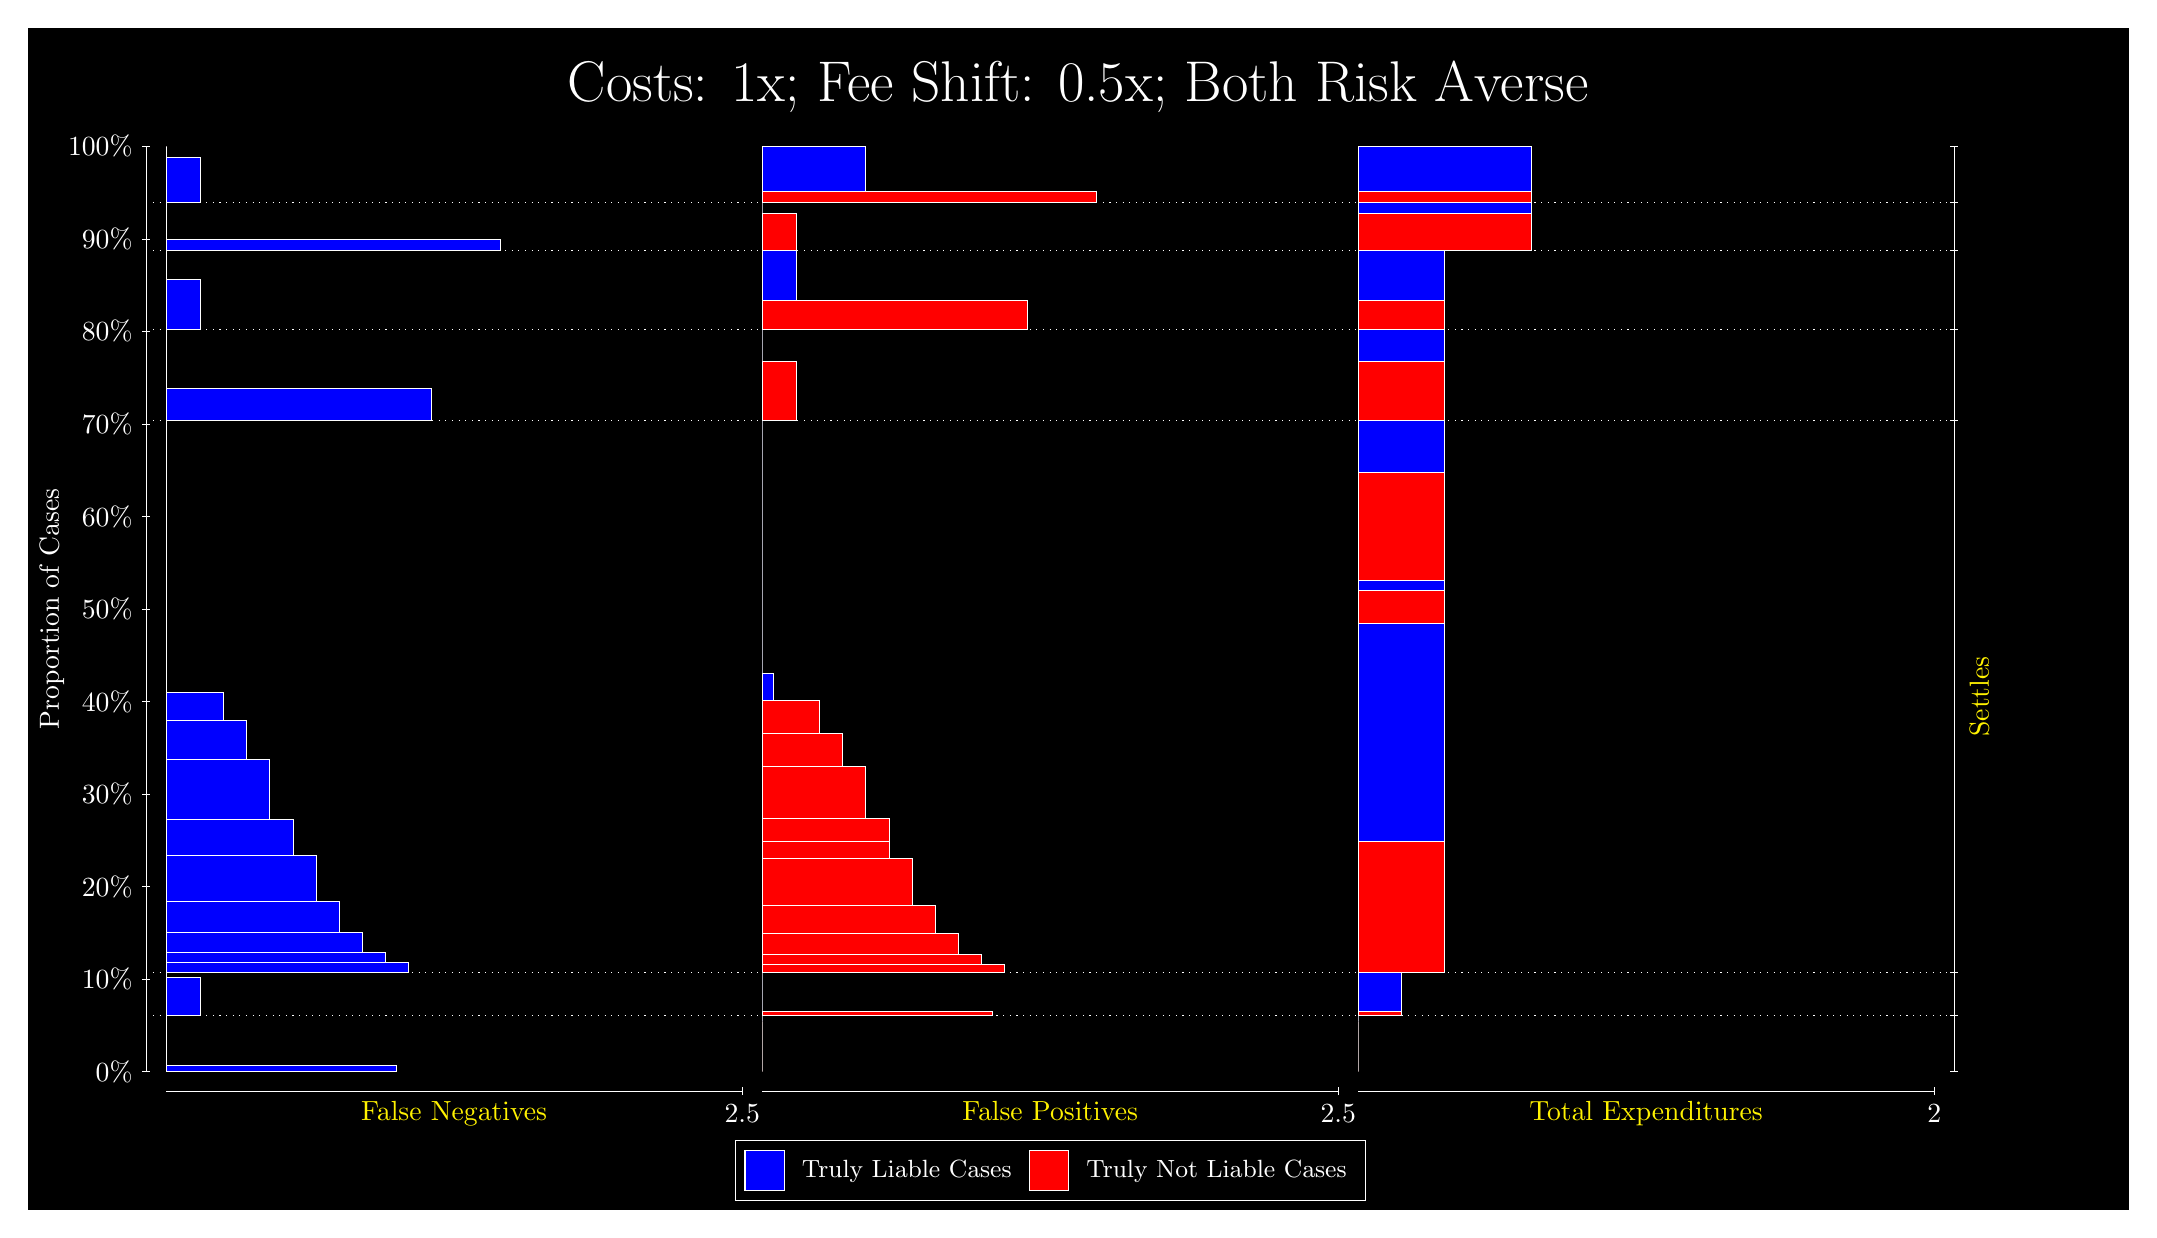
\begin{tikzpicture}
\draw[fill=black] (0,0) rectangle (26.667,15);
\draw[text=white] (0,13.5) rectangle (26.667,15) node[midway] {\huge Costs: 1x; Fee Shift: 0.5x; Both Risk Averse};
\draw[white, very thin] (1.5,1.75) -- (1.5,13.5);
\node[rotate=90, text=white, anchor=center] at (0.3, 7.625) {Proportion of Cases};
\draw[white, very thin] (1.45,1.75) -- (1.55,1.75);
\node[text=white, anchor=east] at (1.45, 1.75) {0\%};
\draw[white, very thin] (1.45,2.925) -- (1.55,2.925);
\node[text=white, anchor=east] at (1.45, 2.925) {10\%};
\draw[white, very thin] (1.45,4.1) -- (1.55,4.1);
\node[text=white, anchor=east] at (1.45, 4.1) {20\%};
\draw[white, very thin] (1.45,5.275) -- (1.55,5.275);
\node[text=white, anchor=east] at (1.45, 5.275) {30\%};
\draw[white, very thin] (1.45,6.45) -- (1.55,6.45);
\node[text=white, anchor=east] at (1.45, 6.45) {40\%};
\draw[white, very thin] (1.45,7.625) -- (1.55,7.625);
\node[text=white, anchor=east] at (1.45, 7.625) {50\%};
\draw[white, very thin] (1.45,8.8) -- (1.55,8.8);
\node[text=white, anchor=east] at (1.45, 8.8) {60\%};
\draw[white, very thin] (1.45,9.975) -- (1.55,9.975);
\node[text=white, anchor=east] at (1.45, 9.975) {70\%};
\draw[white, very thin] (1.45,11.15) -- (1.55,11.15);
\node[text=white, anchor=east] at (1.45, 11.15) {80\%};
\draw[white, very thin] (1.45,12.325) -- (1.55,12.325);
\node[text=white, anchor=east] at (1.45, 12.325) {90\%};
\draw[white, very thin] (1.45,13.5) -- (1.55,13.5);
\node[text=white, anchor=east] at (1.45, 13.5) {100\%};

\draw[white, very thin] (24.457,1.75) -- (24.457,13.5);
\draw[white, very thin] (24.407,1.75) -- (24.507,1.75);
\node[anchor=west] at (24.407, 1.75) {};
\draw[white, very thin] (24.407,2.4628) -- (24.507,2.4628);
\node[anchor=west] at (24.407, 2.4628) {};
\draw[white, very thin] (24.407,3.0059) -- (24.507,3.0059);
\node[anchor=west] at (24.407, 3.0059) {};
\draw[white, very thin] (24.407,10.018) -- (24.507,10.018);
\node[anchor=west] at (24.407, 10.018) {};
\draw[white, very thin] (24.407,11.175) -- (24.507,11.175);
\node[anchor=west] at (24.407, 11.175) {};
\draw[white, very thin] (24.407,12.182) -- (24.507,12.182);
\node[anchor=west] at (24.407, 12.182) {};
\draw[white, very thin] (24.407,12.791) -- (24.507,12.791);
\node[anchor=west] at (24.407, 12.791) {};
\draw[white, very thin] (24.407,13.5) -- (24.507,13.5);
\node[anchor=west] at (24.407, 13.5) {};

\draw[white, very thin, fill=blue] (1.75,1.75) rectangle (4.6775,1.825);
\draw[white, very thin, fill=red] (1.75,1.825) rectangle (1.75,2.4628);
\draw[white, very thin, fill=blue] (1.75,2.4628) rectangle (2.1891,2.9492);
\draw[white, very thin, fill=red] (1.75,2.9492) rectangle (1.75,3.0059);
\draw[white, very thin, fill=blue] (1.75,3.0059) rectangle (4.8239,3.1347);
\draw[white, very thin, fill=blue] (1.75,3.1347) rectangle (4.5312,3.2671);
\draw[white, very thin, fill=blue] (1.75,3.2671) rectangle (4.2384,3.5175);
\draw[white, very thin, fill=blue] (1.75,3.5175) rectangle (3.9457,3.9061);
\draw[white, very thin, fill=blue] (1.75,3.9061) rectangle (3.6529,4.4976);
\draw[white, very thin, fill=blue] (1.75,4.4976) rectangle (3.3602,4.9519);
\draw[white, very thin, fill=blue] (1.75,4.9519) rectangle (3.0674,5.7154);
\draw[white, very thin, fill=blue] (1.75,5.7154) rectangle (2.7746,6.2144);
\draw[white, very thin, fill=blue] (1.75,6.2144) rectangle (2.4819,6.5643);
\draw[white, very thin, fill=red] (1.75,6.5643) rectangle (1.75,10.018);
\draw[white, very thin, fill=blue] (1.75,10.018) rectangle (5.1167,10.429);
\draw[white, very thin, fill=red] (1.75,10.429) rectangle (1.75,11.175);
\draw[white, very thin, fill=blue] (1.75,11.175) rectangle (2.1891,11.81);
\draw[white, very thin, fill=red] (1.75,11.81) rectangle (1.75,12.182);
\draw[white, very thin, fill=blue] (1.75,12.182) rectangle (5.9949,12.318);
\draw[white, very thin, fill=red] (1.75,12.318) rectangle (1.75,12.791);
\draw[white, very thin, fill=blue] (1.75,12.791) rectangle (2.1891,13.363);
\draw[white, very thin, fill=red] (1.75,13.363) rectangle (1.75,13.5);
\draw[white, very thin, fill=red] (9.3189,1.75) rectangle (9.3189,2.3878);
\draw[white, very thin, fill=blue] (9.3189,2.3878) rectangle (9.3189,2.4628);
\draw[white, very thin, fill=red] (9.3189,2.4628) rectangle (12.246,2.5194);
\draw[white, very thin, fill=blue] (9.3189,2.5194) rectangle (9.3189,3.0059);
\draw[white, very thin, fill=red] (9.3189,3.0059) rectangle (12.393,3.1078);
\draw[white, very thin, fill=red] (9.3189,3.1078) rectangle (12.1,3.2403);
\draw[white, very thin, fill=red] (9.3189,3.2403) rectangle (11.807,3.5077);
\draw[white, very thin, fill=red] (9.3189,3.5077) rectangle (11.515,3.8583);
\draw[white, very thin, fill=red] (9.3189,3.8583) rectangle (11.222,4.4607);
\draw[white, very thin, fill=red] (9.3189,4.4607) rectangle (10.929,4.6717);
\draw[white, very thin, fill=red] (9.3189,4.6717) rectangle (10.929,4.9655);
\draw[white, very thin, fill=red] (9.3189,4.9655) rectangle (10.636,5.6225);
\draw[white, very thin, fill=red] (9.3189,5.6225) rectangle (10.344,6.0497);
\draw[white, very thin, fill=red] (9.3189,6.0497) rectangle (10.051,6.4594);
\draw[white, very thin, fill=blue] (9.3189,6.4594) rectangle (9.4652,6.8093);
\draw[white, very thin, fill=blue] (9.3189,6.8093) rectangle (9.3189,10.018);
\draw[white, very thin, fill=red] (9.3189,10.018) rectangle (9.758,10.764);
\draw[white, very thin, fill=blue] (9.3189,10.764) rectangle (9.3189,11.175);
\draw[white, very thin, fill=red] (9.3189,11.175) rectangle (12.686,11.547);
\draw[white, very thin, fill=blue] (9.3189,11.547) rectangle (9.758,12.182);
\draw[white, very thin, fill=red] (9.3189,12.182) rectangle (9.758,12.655);
\draw[white, very thin, fill=blue] (9.3189,12.655) rectangle (9.3189,12.791);
\draw[white, very thin, fill=red] (9.3189,12.791) rectangle (13.564,12.927);
\draw[white, very thin, fill=blue] (9.3189,12.927) rectangle (10.636,13.5);
\draw[white, very thin, fill=red] (16.888,1.75) rectangle (16.888,2.3878);
\draw[white, very thin, fill=blue] (16.888,2.3878) rectangle (16.888,2.4628);
\draw[white, very thin, fill=red] (16.888,2.4628) rectangle (17.437,2.5194);
\draw[white, very thin, fill=blue] (16.888,2.5194) rectangle (17.437,3.0059);
\draw[white, very thin, fill=red] (16.888,3.0059) rectangle (17.986,4.6717);
\draw[white, very thin, fill=blue] (16.888,4.6717) rectangle (17.986,7.4471);
\draw[white, very thin, fill=red] (16.888,7.4471) rectangle (17.986,7.8568);
\draw[white, very thin, fill=blue] (16.888,7.8568) rectangle (17.986,7.9856);
\draw[white, very thin, fill=red] (16.888,7.9856) rectangle (17.986,9.3636);
\draw[white, very thin, fill=blue] (16.888,9.3636) rectangle (17.986,10.018);
\draw[white, very thin, fill=red] (16.888,10.018) rectangle (17.986,10.764);
\draw[white, very thin, fill=blue] (16.888,10.764) rectangle (17.986,11.175);
\draw[white, very thin, fill=red] (16.888,11.175) rectangle (17.986,11.547);
\draw[white, very thin, fill=blue] (16.888,11.547) rectangle (17.986,12.182);
\draw[white, very thin, fill=red] (16.888,12.182) rectangle (19.083,12.655);
\draw[white, very thin, fill=blue] (16.888,12.655) rectangle (19.083,12.791);
\draw[white, very thin, fill=red] (16.888,12.791) rectangle (19.083,12.927);
\draw[white, very thin, fill=blue] (16.888,12.927) rectangle (19.083,13.5);
\draw[white, dotted] (1.5,2.4628) -- (24.457,2.4628);
\draw[white, dotted] (1.5,3.0059) -- (24.457,3.0059);
\draw[white, dotted] (1.5,10.018) -- (24.457,10.018);
\draw[white, dotted] (1.5,11.175) -- (24.457,11.175);
\draw[white, dotted] (1.5,12.182) -- (24.457,12.182);
\draw[white, dotted] (1.5,12.791) -- (24.457,12.791);
\draw[white, very thin] (1.75,1.5) -- (9.0689,1.5);
\node[text=yellow, anchor=north] at (5.4094, 1.5) {False Negatives};
\draw[white, very thin] (9.0689,1.45) -- (9.0689,1.55);
\node[text=white, anchor=north] at (9.0689, 1.45) {2.5};

\draw[white, very thin] (9.3189,1.5) -- (16.638,1.5);
\node[text=yellow, anchor=north] at (12.978, 1.5) {False Positives};
\draw[white, very thin] (16.638,1.45) -- (16.638,1.55);
\node[text=white, anchor=north] at (16.638, 1.45) {2.5};

\draw[white, very thin] (16.888,1.5) -- (24.207,1.5);
\node[text=yellow, anchor=north] at (20.547, 1.5) {Total Expenditures};
\draw[white, very thin] (24.207,1.45) -- (24.207,1.55);
\node[text=white, anchor=north] at (24.207, 1.45) {2};



\node[text=yellow, centered, rotate=90] at (24.777, 6.5118) {Settles};





\draw (12.978300999999998,1.5) node[draw=none] (baseCoordinate) {};
\begin{scope}[align=center]
        \matrix[scale=0.5, draw=white, below=0.5cm of baseCoordinate, nodes={draw}, column sep=0.1cm]{
            \node[rectangle, draw, minimum width=0.5cm, minimum height=0.5cm, fill=blue] {}; &
            \node[draw=none, font=\small, text=white] (B) {Truly Liable Cases}; &
            \node[rectangle, draw, minimum width=0.5cm, minimum height=0.5cm, fill=red] {}; &
            \node[draw=none, font=\small, text=white] (B) {Truly Not Liable Cases}; \\
            };
\end{scope}

\end{tikzpicture}
\end{document}